\documentclass[a4paper, 14pt]{extarticle}

% Поля
%--------------------------------------
\usepackage{geometry}
\geometry{a4paper,tmargin=2cm,bmargin=2cm,lmargin=3cm,rmargin=1cm}
%--------------------------------------


%Russian-specific packages
%--------------------------------------
\usepackage[T2A]{fontenc}
\usepackage[utf8]{inputenc} 
\usepackage[english, main=russian]{babel}
%--------------------------------------

\usepackage{textcomp}

% Красная строка
%--------------------------------------
\usepackage{indentfirst}               
%--------------------------------------             


%Graphics
%--------------------------------------
\usepackage{graphicx}
\graphicspath{ {./images/} }
\usepackage{wrapfig}
%--------------------------------------

% Полуторный интервал
%--------------------------------------
\linespread{1.3}                    
%--------------------------------------

%Выравнивание и переносы
%--------------------------------------
% Избавляемся от переполнений
\sloppy
% Запрещаем разрыв страницы после первой строки абзаца
\clubpenalty=10000
% Запрещаем разрыв страницы после последней строки абзаца
\widowpenalty=10000
%--------------------------------------

%Списки
\usepackage{enumitem}

%Подписи
\usepackage{caption} 

%Гиперссылки
\usepackage{hyperref}

\hypersetup {
	unicode=true
}

%Рисунки
%--------------------------------------
\DeclareCaptionLabelSeparator*{emdash}{~--- }
\captionsetup[figure]{labelsep=emdash,font=onehalfspacing,position=bottom}
%--------------------------------------

\usepackage{tempora}

%Листинги
%--------------------------------------
\usepackage{listings}
\lstset{
  basicstyle=\ttfamily\footnotesize, 
  %basicstyle=\footnotesize\AnkaCoder,        % the size of the fonts that are used for the code
  breakatwhitespace=false,         % sets if automatic breaks shoulbd only happen at whitespace
  breaklines=true,                 % sets automatic line breaking
  captionpos=t,                    % sets the caption-position to bottom
  inputencoding=utf8,
  frame=single,                    % adds a frame around the code
  keepspaces=true,                 % keeps spaces in text, useful for keeping indentation of code (possibly needs columns=flexible)
  keywordstyle=\bf,       % keyword style
  numbers=left,                    % where to put the line-numbers; possible values are (none, left, right)
  numbersep=5pt,                   % how far the line-numbers are from the code
  xleftmargin=25pt,
  xrightmargin=25pt,
  showspaces=false,                % show spaces everywhere adding particular underscores; it overrides 'showstringspaces'
  showstringspaces=false,          % underline spaces within strings only
  showtabs=false,                  % show tabs within strings adding particular underscores
  stepnumber=1,                    % the step between two line-numbers. If it's 1, each line will be numbered
  tabsize=2,                       % sets default tabsize to 8 spaces
  title=\lstname                   % show the filename of files included with \lstinputlisting; also try caption instead of title
}
%--------------------------------------

%%% Математические пакеты %%%
%--------------------------------------
\usepackage{amsthm,amsfonts,amsmath,amssymb,amscd}  % Математические дополнения от AMS
\usepackage{mathtools}                              % Добавляет окружение multlined
\usepackage[perpage]{footmisc}
%--------------------------------------

%--------------------------------------
%			НАЧАЛО ДОКУМЕНТА
%--------------------------------------

\begin{document}

%--------------------------------------
%			ТИТУЛЬНЫЙ ЛИСТ
%--------------------------------------
\begin{titlepage}
\thispagestyle{empty}
\newpage


%Шапка титульного листа
%--------------------------------------
\vspace*{-60pt}
\hspace{-65pt}
\begin{minipage}{0.3\textwidth}
\hspace*{-20pt}\centering

\includegraphics[width=\textwidth]{emblem}
\end{minipage}
\begin{minipage}{0.67\textwidth}\small \textbf{
\vspace*{-0.7ex}
\hspace*{-6pt}\centerline{Министерство науки и высшего образования Российской Федерации}
\vspace*{-0.7ex}
\centerline{Федеральное государственное бюджетное образовательное учреждение }
\vspace*{-0.7ex}
\centerline{высшего образования}
\vspace*{-0.7ex}
\centerline{<<Московский государственный технический университет}
\vspace*{-0.7ex}
\centerline{имени Н.Э. Баумана}
\vspace*{-0.7ex}
\centerline{(национальный исследовательский университет)>>}
\vspace*{-0.7ex}
\centerline{(МГТУ им. Н.Э. Баумана)}}
\end{minipage}
%--------------------------------------

%Полосы
%--------------------------------------
\vspace{-25pt}
\hspace{-35pt}\rule{\textwidth}{2.3pt}

\vspace*{-20.3pt}
\hspace{-35pt}\rule{\textwidth}{0.4pt}
%--------------------------------------

\vspace{1.5ex}
\hspace{-35pt} \noindent \small ФАКУЛЬТЕТ\hspace{80pt} <<Информатика и системы управления>>

\vspace*{-16pt}
\hspace{47pt}\rule{0.83\textwidth}{0.4pt}

\vspace{0.5ex}
\hspace{-35pt} \noindent \small КАФЕДРА\hspace{50pt} <<Теоретическая информатика и компьютерные технологии>>

\vspace*{-16pt}
\hspace{30pt}\rule{0.866\textwidth}{0.4pt}
  
\vspace{11em}

\begin{center}
\Large {\bf Лабораторная работа № 3} \\ 
\large {\bf по курсу <<Компьютерные сети>>} \\
\large <<Протокол одноранговой сети>> 
\end{center}\normalsize

\vspace{8em}


\begin{flushright}
  {Студент группы ИУ9-32Б Волохов А. В. \hspace*{15pt}\\ 
  \vspace{2ex}
  Преподаватель Посевин Д. П.\hspace*{15pt}}
\end{flushright}

\bigskip

\vfill
 

\begin{center}
\textsl{Москва 2023}
\end{center}
\end{titlepage}
%--------------------------------------
%		КОНЕЦ ТИТУЛЬНОГО ЛИСТА
%--------------------------------------

\renewcommand{\ttdefault}{pcr}

\setlength{\tabcolsep}{3pt}
\newpage
\setcounter{page}{2}
\section{Задание}\label{Sect::task}
Целью данной работы является разработка одноранговой сетевой службы.
Распределённая хеш-таблица (полносвязная)
Топология: полносвязная.
Информация, известная пиру при запуске: его IP-адрес и порт,
а также IP-адреса и порты возможных соседей.
Описание службы: каждый пир через стандартный поток
ввода принимает команды – добавить пару «ключ–значение»,
удалить пару по ключу, найти значение по ключу.
Замечание: все словарные пары доступны всем пирам; позже
добавленные пары должны замещать ранее добавленные пары
с тем же ключом
Исходный код программы представлен в листингах~\ref{lst:code1}--~\ref{lst:code2}--~\ref{lst:code3}--~\ref{lst:code4}--~\ref{lst:code5}--~\ref{lst:code6}.

\begin{figure}[!htb]
\begin{lstlisting}[language={Go},caption={acces.go},label={lst:code1}]
package main

import (
	"bufio"
	"encoding/json"
	"fmt"
	"net"
	"os"
	"strings"
)

type Message struct {
	Command string `json:"command"`
	Key     string `json:"key"`
	Value   string `json:"value"`
	IP      string `json:"ip"`
	Port    string `json:"port"`
	Forward bool   `json:"forward"`
}

func main() {
	var peerAddress string
	var conn net.Conn
	var err error
	scanner := bufio.NewScanner(os.Stdin)
	for {
		fmt.Print("Enter a command: ")
		scanner.Scan()
		command := scanner.Text()

		if command == "exit" {
			break
		}

		parts := strings.Fields(command)
		if parts[0] == "PEER" && len(parts) == 2 {
			peerAddress = parts[1]
			conn, err = net.Dial("tcp", peerAddress)
			if err != nil {
				fmt.Printf("Error: %s\n", err)
				continue
			}
			fmt.Println("Connected to peer:", peerAddress)
		} else if parts[0] == "ADD_NEIGHBOR" && len(parts) == 3 {
			msg := Message{
				Command: "ADD_NEIGHBOR",
				IP:      parts[1],
				Port:    parts[2],
			}

			msgBytes, err := json.Marshal(msg)
			if err != nil {
				fmt.Printf("Error encoding message: %s\n", err)
				continue
			}
			_, err = conn.Write(append(msgBytes, '\n'))
			if err != nil {
				fmt.Printf("Error sending message: %s\n", err)
			}
		} 

\end{lstlisting}
\end{figure}

\newpage

\begin{figure}[!htb]
\begin{lstlisting}[language={Go},caption={acces.go - продолжение},label={lst:code2}]
else if conn != nil {
			msg := Message{
				Command: parts[0],
				Key:     "",
				Value:   "",
			}

			if len(parts) > 1 {
				msg.Key = parts[1]
			}

			if len(parts) > 2 {
				msg.Value = parts[2]
			}

			msgBytes, err := json.Marshal(msg)
			if err != nil {
				fmt.Printf("Error encoding message: %s\n", err)
				continue
			}
			_, err = conn.Write(append(msgBytes, '\n'))
			if err != nil {
				fmt.Printf("Error sending message: %s\n", err)
			}
		} else {
			fmt.Println("You must first connect to a peer using 'PEER <port>'")
		}
	}

	if conn != nil {
		err := conn.Close()
		if err != nil {
			return
		}
	}
}

\end{lstlisting}
\end{figure}

\newpage
\begin{figure}[!htb]
\begin{lstlisting}[language={Go},caption={peer.go},label={lst:code3}]
package main

import (
	"bufio"
	"encoding/json"
	"fmt"
	"net"
	"os"
	"sync"
)

type HashTable struct {
	data  map[string]string
	mutex sync.Mutex
}

type Neighbor struct {
	IP   string
	Port string
}

type Message struct {
	Command string `json:"command"`
	Key     string `json:"key"`
	Value   string `json:"value"`
	IP      string `json:"ip"`
	Port    string `json:"port"`
	Forward bool   `json:"forward"`
}

func (h *HashTable) Add(key, value string) {
	h.mutex.Lock()
	defer h.mutex.Unlock()
	h.data[key] = value
}

func (h *HashTable) Delete(key string) {
	h.mutex.Lock()
	defer h.mutex.Unlock()
	delete(h.data, key)
}

func (h *HashTable) Find(key string) string {
	h.mutex.Lock()
	defer h.mutex.Unlock()
	if val, found := h.data[key]; found {
		return val
	}
	return "Key not found"
}
\end{lstlisting}
\end{figure}
\newpage
\begin{figure}[!htb]
\begin{lstlisting}[language={Go},caption={peer.go - продолжение},label={lst:code4}]
func main() {
	// Создаем и инициализируем хеш-таблицу
	hashTable := &HashTable{
		data: make(map[string]string),
	}

	// Слайс для хранения информации о соседях
	neighbors := make([]Neighbor, 0)

	// Первый аргумент командной строки - порт, на котором данный пир будет слушать
	if len(os.Args) != 2 {
		fmt.Println("Usage: go run peer.go <port>")
		return
	}

	// Получаем порт из аргументов командной строки
	port := os.Args[1]

	// Запуск слушающего сервера
	listener, err := net.Listen("tcp", ":"+port)
	if err != nil {
		fmt.Printf("Error: %s\n", err)
		return
	}
	defer func(listener net.Listener) {
		err := listener.Close()
		if err != nil {

		}
	}(listener)

	fmt.Printf("Peer listening on port %s\n", port)

	for {
		conn, err := listener.Accept()
		if err != nil {
			fmt.Printf("Error: %s\n", err)
			continue
		}

		go handleConnection(conn, hashTable, &neighbors)
	}
}

func handleConnection(conn net.Conn, hashTable *HashTable, neighbors *[]Neighbor) {
	defer func(conn net.Conn) {
		err := conn.Close()
		if err != nil {

		}
	}(conn)

	// Получение IP и порта соседа
\end{lstlisting}
\end{figure}
\newpage
\begin{figure}[!htb]
\begin{lstlisting}[language={Go},caption={peer.go - продолжение},label={lst:code5}]
remoteAddr := conn.RemoteAddr().String()
	fmt.Printf("Connected to peer at %s\n", remoteAddr)

	scanner := bufio.NewScanner(conn)
	for scanner.Scan() {
		command := scanner.Text()

		// Распаковка JSON-сообщения
		var msg Message
		err := json.Unmarshal([]byte(command), &msg)
		if err != nil {
			fmt.Printf("Error decoding message: %s\n", err)
			continue
		}

		switch msg.Command {
		case "ADD":
			if msg.Key != "" && msg.Value != "" {
				hashTable.Add(msg.Key, msg.Value)
				fmt.Printf("Added key-value pair: %s-%s\n", msg.Key, msg.Value)
				if !msg.Forward {
					// Отправляем запрос всем соседям, исключая отправителя
					for _, neighbor := range *neighbors {
						if neighbor.IP != msg.IP || neighbor.Port != msg.Port {
							sendRequest(neighbor.IP, neighbor.Port, msg)
						}
					}
				}
			}
		case "DELETE":
			if msg.Key != "" {
				hashTable.Delete(msg.Key)
				fmt.Printf("Deleted key: %s\n", msg.Key)
				if !msg.Forward {
					// Отправляем запрос всем соседям, исключая отправителя
					for _, neighbor := range *neighbors {
						if neighbor.IP != msg.IP || neighbor.Port != msg.Port {
							sendRequest(neighbor.IP, neighbor.Port, msg)
						}
					}
				}
			}
		case "FIND":
			if msg.Key != "" {
				value := hashTable.Find(msg.Key)
				fmt.Printf("Found value: %s\n", value)
			}
		case "LIST_NEIGHBORS":
			// Вывод информации о соседях в стандартный вывод
			fmt.Println("List of neighbors:")
			for _, neighbor := range *neighbors {
				fmt.Printf("IP: %s, Port: %s\n", neighbor.IP, neighbor.Port)
			}
\end{lstlisting}
\end{figure}

\newpage

\begin{figure}[!htb]
\begin{lstlisting}[language={Go},caption={peer.go - продолжение},label={lst:code6}]
case "ADD_NEIGHBOR":
			// Добавляем соседа
			if msg.IP != "" && msg.Port != "" {
				*neighbors = append(*neighbors, Neighbor{IP: msg.IP, Port: msg.Port})
				fmt.Printf("Added neighbor: %s:%s\n", msg.IP, msg.Port)
			}
		}
	}
}

func sendRequest(ip, port string, msg Message) {
	msg.Forward = true
	msg.IP = ""
	msg.Port = ""
	neighborAddr := ip + ":" + port
	conn, err := net.Dial("tcp", neighborAddr)
	if err != nil {
		fmt.Printf("Error connecting to neighbor %s: %s\n", neighborAddr, err)
		return
	}
	defer func(conn net.Conn) {
		err := conn.Close()
		if err != nil {

		}
	}(conn)
	msgBytes, err := json.Marshal(msg)
	if err != nil {
		fmt.Printf("Error encoding message: %s\n", err)
		return
	}
	_, err = conn.Write(append(msgBytes, '\n'))
	if err != nil {
		fmt.Printf("Error sending message to neighbor %s: %s\n", neighborAddr, err)
		return
	}
}

\end{lstlisting}
\end{figure}

\newpage

\begin{figure}[!htb]
	\centering
	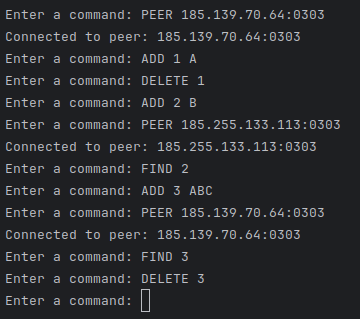
\includegraphics[width=0.8\textwidth]{res1.png}
\caption{Клиент}
\label{fig:img1}
\end{figure}
\begin{figure}[!htb]
	\centering
	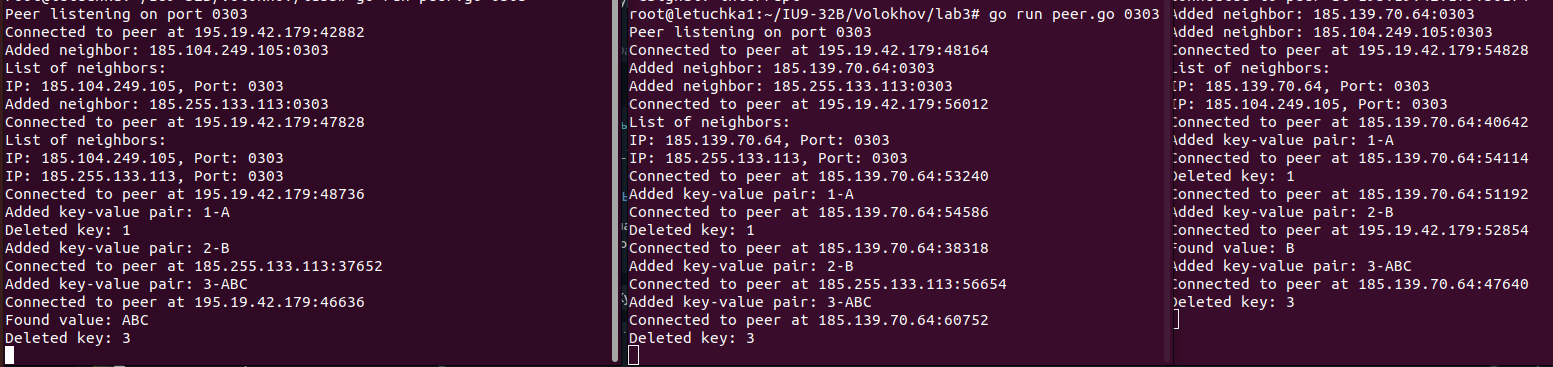
\includegraphics[width=0.8\textwidth]{res2.png}
\caption{Сервер}
\label{fig:img2}
\end{figure}





\end{document}
